\chapter{Development Methodology}

\section{Initial Project Plan}
As the project began, the group had a number of meetings in quick succession in order to come up with an initial plan.  One major point on the agenda was the development methodology to use - many group members wanted to take an agile approach, but were unsure of which flavour of agile to adopt.  After evaluating the most commonly used approaches, the \textit{Scrumban}\cite{scrumban} methodology was chosen.  \textit{Scrumban} combines the benefits of the Scrum and Kanban methodologies, allowing the group to split into smaller sub-groups to tackle individual services, visualise the outstanding work, and respond quickly to requirements changes. Additionally, \textit{Scrumban} is tailored for the difficulties around estimating each sprint or the current velocity, which would be particularly useful as nobody within the group had any experience with the required application frameworks, Java EE and .NET Core. 

There were initially nine distinct microservices identified which would be required in order to meet the functional requirements.  Services were designated with a language in which they would be implemented. (Fig. \ref{fig:initial_spec_chart})

\begin{figure}[H]
    \centering
    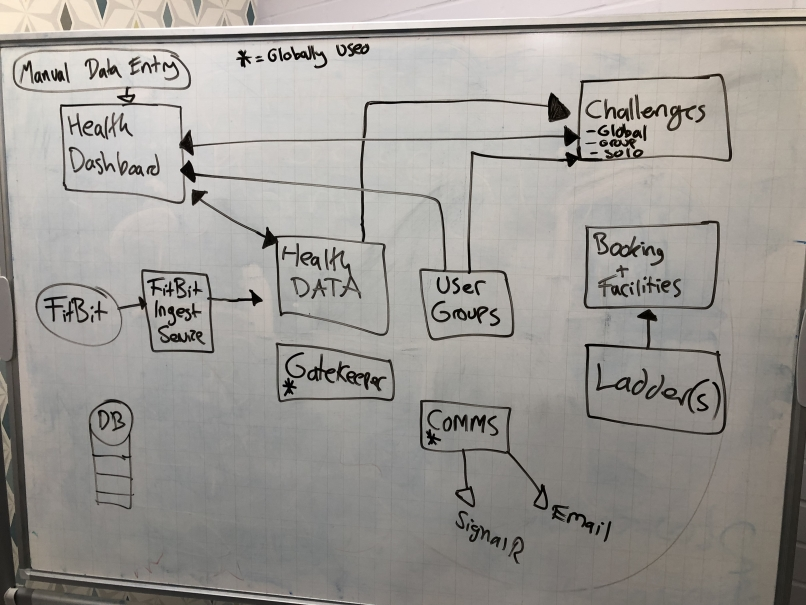
\includegraphics[width=\textwidth]{Images/Initial_Spec_Chart.jpg}
    \caption{Initial design diagram identifying the nine microservices and interactions between them.}
    \label{fig:initial_spec_chart}
\end{figure}

Microservices were designated with a priority ranking between 1 and 3(Fig. \ref{fig:numbering_microservice_priority}).  Services which were critical to the core functionality of the entire system were assigned a priority of 1, an example of which is \textit{Health Data Repository} which is responsible for the central storage of all activity data within the system.  Services with less crucial functionality were assigned priority 2 or 3 as appropriate.

\begin{figure}[H]
    \centering
    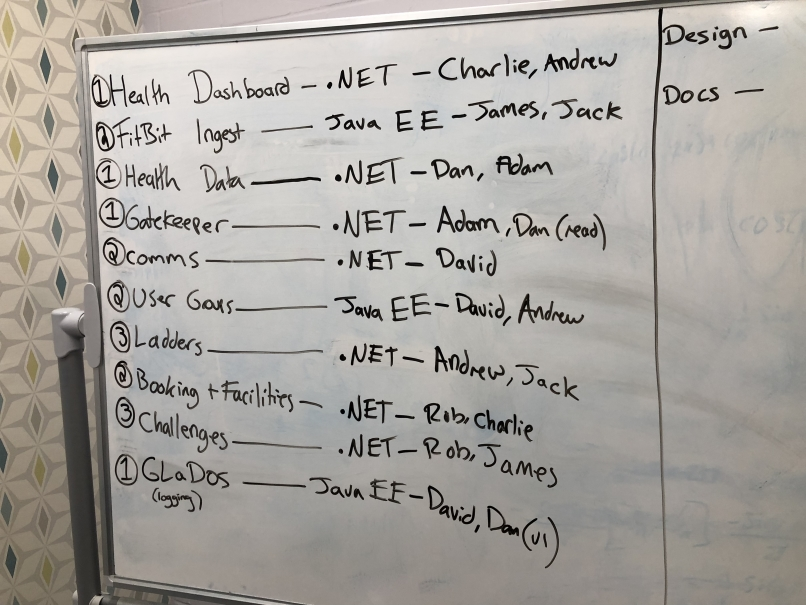
\includegraphics[width=\textwidth]{Images/Numbering_Microservices.jpg}
    \caption{Microservice prioritisation and developer assignment}
    \label{fig:numbering_microservice_priority}
\end{figure}


\section{Supporting Tools}
\subsection{GitHub \& TravisCI}
\textit{GitHub}\footnote{https://github.com/sem5640-2018} was chosen as the version control host for all repositories, due to the vast array of features and tooling supported by the platform.  The use of \textit{GitHub} allowed easy integration with \textit{Travis CI} to automatically trigger the running of unit tests and the building of \textit{Docker} images, and additionally allowed the enforcement of code quality procedures such as requiring peer review of code before merging, and preventing merges of code with failing tests.  Integration with \texit{Slack} provided the group with instant notifications of events such as new pull requests and the status of \texit{Travis CI} builds.

\begin{figure}[H]
    \centering
    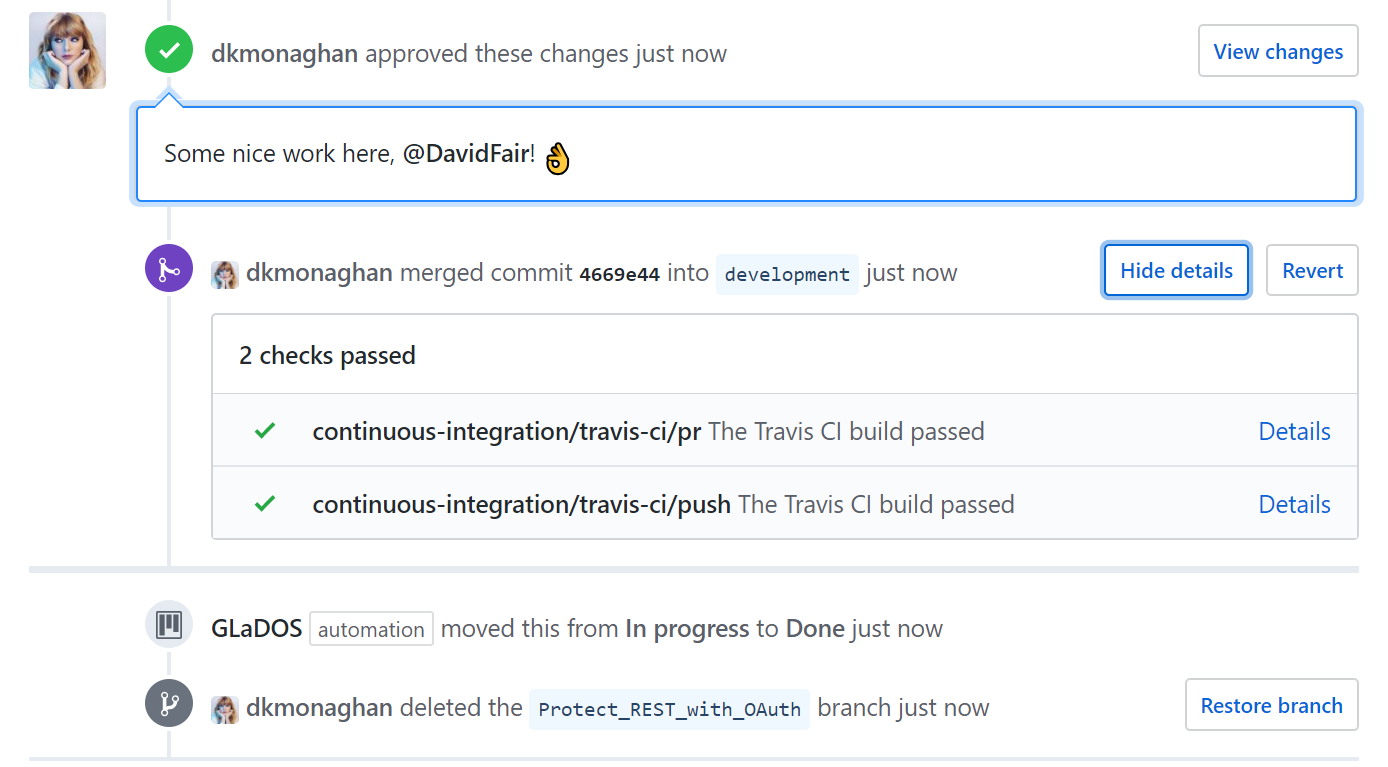
\includegraphics[width=\textwidth]{Images/approve_pr.png}
    \caption{Example of a pull request being peer reviewed. The \textit{TravisCI} builds were successful,allowing the branch to be merged into an upstream branch.}
    \label{fig:approve_pull_request}
\end{figure}

Once a pull request had been approved and merged (Fig. \ref{fig:approve_pull_request}), \textit{TravisCI} would build and push the \textit{Docker} image to \textit{Docker Hub}.

\begin{figure}[H]
    \centering
    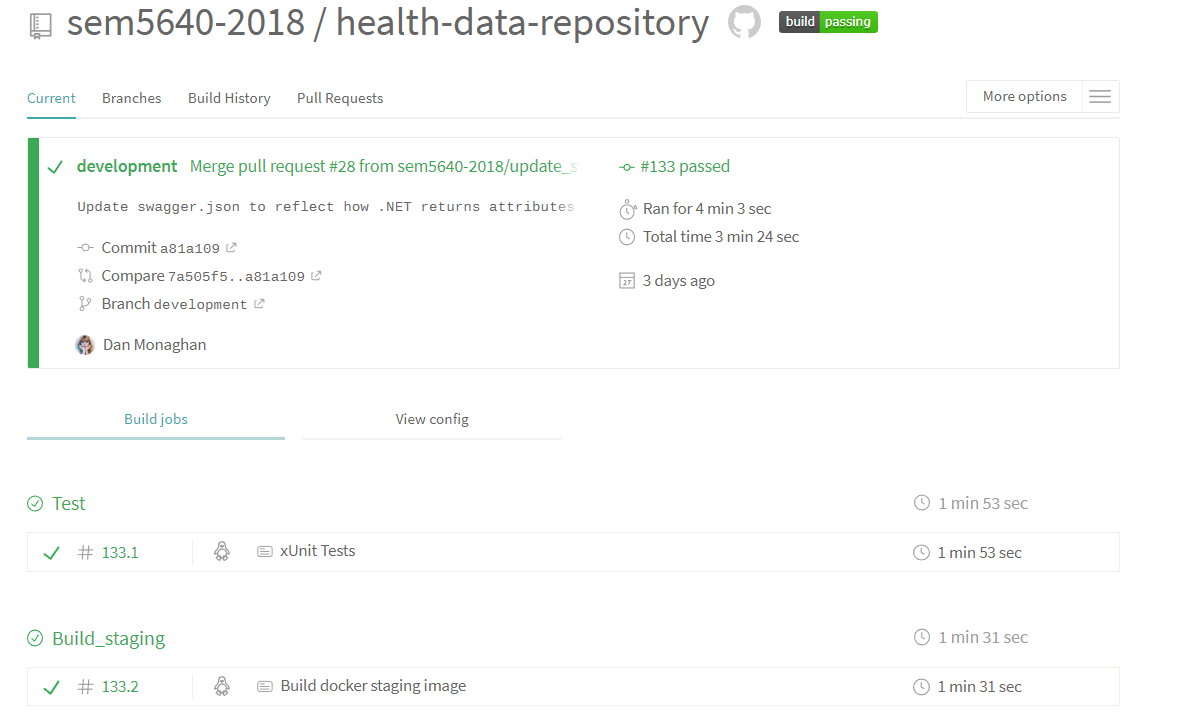
\includegraphics[width=\textwidth]{Images/travis_builds_overview.png}
    \caption{Example of \textit{Travis CI} running unit tests and building a \texit{Docker} image after a successful merge to the development branch.}
    \label{fig:travis_ui}
\end{figure}

\subsection{Swagger}
\begin{figure}[H]
    \centering
    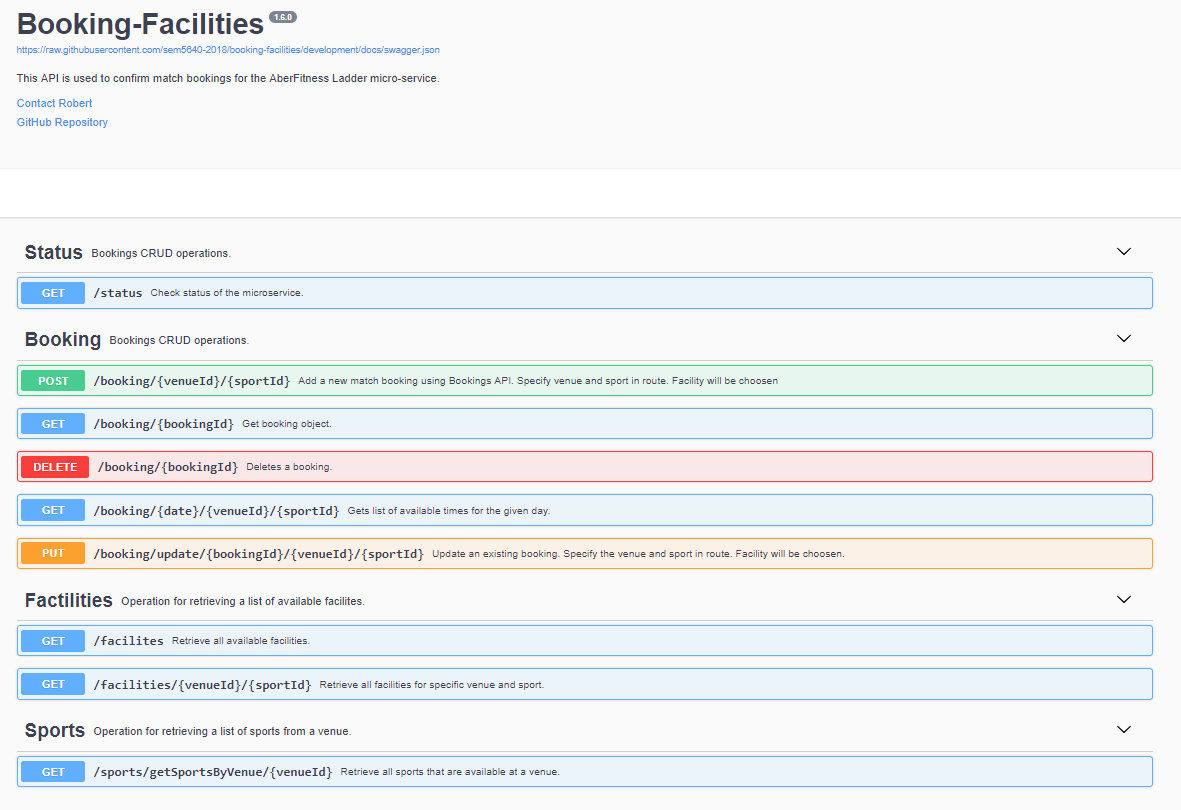
\includegraphics[width=\textwidth]{Images/Swagger.png}
    \caption{The Swagger interface for the \textit{Booking Facilities} microservice}
    \label{fig:swagger_ui}
\end{figure}

\textit{Swagger} is a web based application for documenting API specifications. Each microservice within \textit{Aber Fitness} has a file located in \lstinline{docs/swagger.json} which defines its API endpoints and any associated data models. \textit{Swagger} was a crucial part of the development process as it not only allowed us to draft API specifications, but allowed development of consuming services to happen in parallel, and promote fast feedback should missing functionality be identified.

\subsection{Portainer}
\begin{figure}[H]
    \centering
    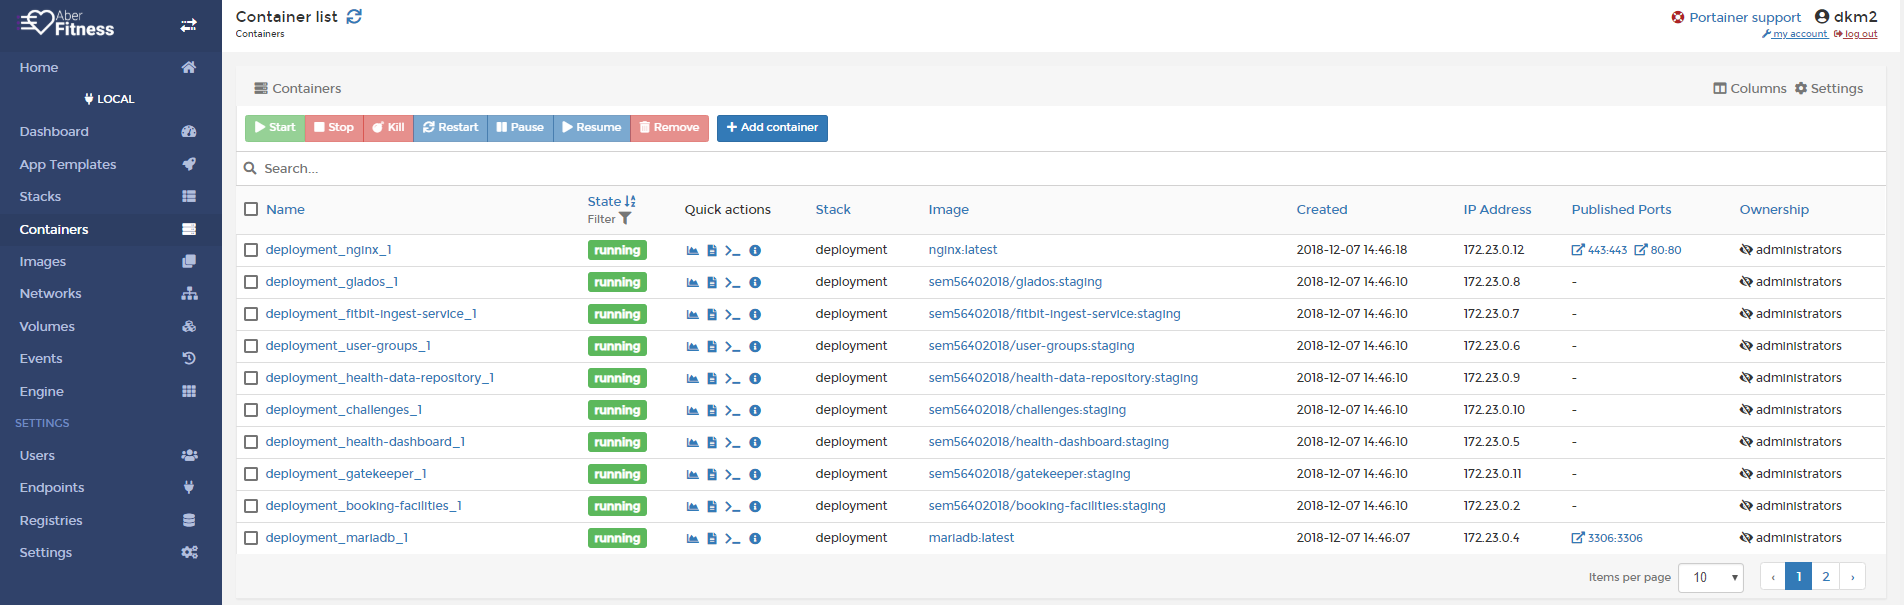
\includegraphics[width=\textwidth]{Images/Portainer.png}
    \caption{The Portainer interface for our staging / development Docker host, \lstinline{docker2-m56.dcs.aber.ac.uk}}
    \label{fig:portainer_ui}
\end{figure}

\textit{Portainer} provides a dashboard for managing \textit{Docker} volumes, networks, images and containers. Whilst completing the initial configuration of the \textit{Docker} images, \textit{Portainer} proved invaluable, as it provided rapid visual feedback allowing developers to quickly and easily debug problems by identifying which services were running, which were not, and allowing easy access to the application console output.

\subsection{Docker Hub}
\textit{Docker Hub} is an online platform provided by \textit{Docker} which allows \textit{Docker} container images to be uploaded and hosted. The image full system stack is defined in the \lstinline{docker-compose} file, which can be updated and re-deployed . As part of our build process (Fig. \ref{fig:development_flow_diagram}), images are built by \textit{TravisCI} and then pushed to \textit{Docker Hub} before being pulled down onto the \textit{Docker} hosts.

\subsection{Slack \& Deployment}
\textit{Slack} is a hosted chat service designed for offices and teams, and particularly suits itself to the development of software. The group used \textit{Slack} extensively throughout the development of \textit{Aber Fitness} not only to communicate and discuss progress, ideas and troubleshoot problems, but also made extensive use of \textit{Slack}'s integrations with services such as \textit{TravisCI} and \textit{GitHub} (Fig. \ref{fig:slack_travis_github})

\begin{figure}[H]
    \centering
    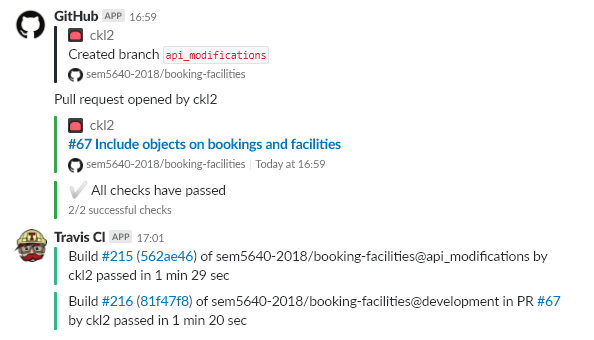
\includegraphics[width=\textwidth]{Images/Slack_Travis_GitHub.png}
    \caption{A screenshot of the \textit{Slack} channel \lstinline{\#dev-booking-facilities} demonstrating the integrations between \textit{Slack}, \textit{GitHub} and \textit{TravisCI}}
    \label{fig:slack_travis_github}
\end{figure}

\textit{Slack} also played a major role in our deployment strategy when rolling out updated \textit{Docker} images to our staging host. On multiple occasions we ran into permission issues whilst trying to deploy on the two \textit{Docker} hosts we had been provided by the Computer Science department. Each member of the team had their own individual login to the hosts, so permissions errors would occur after performing commands like \lstinline{git pull}. 

Another issue we ran into was developers forgetting the specific command sequence to update the application images. This would lead to confusion when the upstream changes were not deployed, wasting valuable development time resolving bugs. (Fig. \ref{fig:david_being_a_dumbass})

\begin{figure}[H]
    \centering
    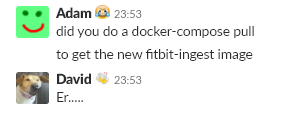
\includegraphics[width=0.5\textwidth]{Images/aberfitness_slack_bot_reason_why.png}
    \caption{An example situation where the execution of \lstinline{docker-compose pull} caused a large amount of confusion amongst \textit{Aber Fitness} developers}
    \label{fig:david_being_a_dumbass}
\end{figure}

\textit{Slack} ended up providing us with an elegant solution to this, users could call a custom webhook by entering a specific command in a chat channel. A \textit{Slack} application was put together to automatically pull the latest \lstinline{docker-compose.yml} file from GitHub, as well as updating all the \textit{Docker Hub} images, then re-deploy the stack. This could all be done from within \textit{Slack} itself through the \lstinline{/deploy} command. (Fig. \ref{fig:slack_bot})

\begin{figure}[H]
    \centering
    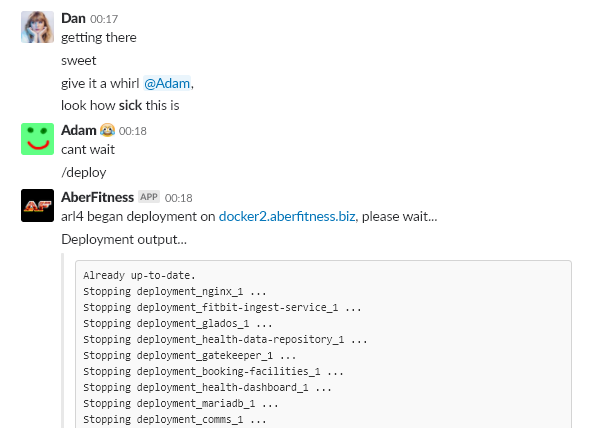
\includegraphics[width=0.9\textwidth]{Images/aberfitness_slack_bot.png}
    \caption{A demonstration of the \lstinline{/deploy} command being used to re-deploy \textit{Aber Fitness} onto the staging host}
    \label{fig:slack_bot}
\end{figure}

